% ==============================================================================
% PLANTILLA MAESTRA - UnADM (instrucciones comunes)
% ==============================================================================
% Uso rapido:
% 1) Duplica la plantilla y renombra la copia por semana/actividad.
% 2) Actualiza \documenttitle, \documentsubtitle y \documentsubject.
% 3) Lee la planeacion y NO pegues las instrucciones completas dentro del PDF.
%    Usa la planeacion como lista de cumplimiento y redacta con criterio propio.
% 4) Elabora productos visuales preferentemente en LaTeX/TikZ para mantener
%    nitidez y evidencia editable; si usas herramientas externas, inserta
%    capturas de alta resolucion y conserva evidencia dentro del PDF.
% 5) Entrega en PDF con la nomenclatura solicitada en el aula.
%
% Formato institucional (recomendado):
% - Fuente: Helvetica / sans-serif equivalente (\usepackage{helvet}).
% - Interlineado: 1.5 (\onehalfspacing).
% - Citas: autor-año mediante natbib (\citep, \citet, \citep[e.g.][]{clave}).
% - Bibliografía: archivo .bib con formato APA 7; todas las citas del texto
%   deben aparecer en la bibliografía y viceversa.
% - Estructura mínima: portada, resumen/abstract, desarrollo, conclusión y
%   bibliografía.
%
% Reglas para productos visuales y tablas extensas:
% - Para tablas o cuadros amplios use longtable + booktabs y evite líneas
%   verticales; controlar espaciado con \setlength{\tabcolsep} y
%   \renewcommand{\arraystretch}.
% - Para tablas en página propia: use \clearpage, \pagestyle{empty},
%   entorno landscape, reducir tamaño con \scriptsize y luego restaurar
%   \pagestyle{fancy} al finalizar la tabla.
%
% Buenas prácticas de redacción académica (guía operativa):
% - No escribir para llenar espacio; escribir para sostener y defender una idea.
% - Cada concepto debe responder: qué es, qué características tiene, cómo
%   funciona, qué problema resuelve, qué límite presenta y qué implicación
%   jurídica posee.
% - Evitar listas sin análisis: tras cada dato relevante incluya su consecuencia
%   o aplicación jurídica.
% - Primera persona: usar moderadamente ("Considero que", "Desde esta
%   perspectiva"); evite expresiones coloquiales como "yo creo".
%
% Protocolos de integridad y uso de IA:
% - Si se usa IA, el resultado debe ser leído, corregido y transformado con
%   criterio propio. No entregar texto sin procesamiento.
% - Incluir siempre juicio propio y referencias que sostengan la postura.
%
% Checklist operativo antes de entregar:
% [ ] El producto coincide con la técnica solicitada en la planeación.
% [ ] El objetivo y el contenido están alineados con la planeación.
% [ ] El producto visual está rotulado y presentado como se pide.
% [ ] Hay citas APA autor-año dentro del texto y bibliografía completa.
% [ ] No se incluyeron instrucciones copiadas de la planeación dentro del
%     contenido entregado.
% [ ] Ortografía y redacción revisadas; la argumentación es propia.
% ==============================================================================

% CREACION DEL DOCUMENTO
\documentclass[
	spanish,
	letterpaper, oneside
]{article}

% ==============================================================================
% INFORMACION DEL DOCUMENTO
% Actualizar en cada actividad.
% Ejemplos:
% \def\documenttitle {Cuadro comparativo de escuelas clasicas de la etica}
% \def\documentsubtitle {Actividad 2 - Etica y Moral juridica}
% \def\documentsubject {Actividad Semana 2}
% ==============================================================================
\def\documenttitle {Análisis de hechos sobre vulneración de derechos humanos en México: caso Ayotzinapa}
\def\documentsubtitle {Actividad 7 - Ética y Moral jurídica}
\def\documentsubject {Semana 8 - Análisis de hechos}

\def\documentauthor {Martín Jonathan de la Cruz}
\def\coursename {Ética y Moral jurídica}
\def\coursecode {030}

\def\universityname {Universidad Abierta y a Distancia de México}
\def\universityfaculty {Licenciatura en Derecho}
\def\universitydepartment {Ética y Moral jurídica}
\def\universitydepartmentimage {departamentos/UnADM}
\def\universitydepartmentimagecfg {height=1.57cm}
\def\universitylocation {Roma Norte, Ciudad de México}

% INTEGRANTES, PROFESORES Y FECHAS
\def\authortable {
	\begin{tabular}{ll}
		\textbf{Alumno:}
		& \begin{tabular}[t]{l}
			 Martín Jonathan de la Cruz \\
		\end{tabular} \\
		Matrícula: & ES2611202040 \\

		\textit{Profesor:}
		& \begin{tabular}[t]{l}
			Emma Liliana \\ Padilla Cano
		\end{tabular} \\
		& \\
		\multicolumn{2}{l}{Fecha de realización: \today} \\
		\multicolumn{2}{l}{\universitylocation}
	\end{tabular}
}

% IMPORTACION DEL TEMPLATE
\input{template}

% FORMATO SOLICITADO / USADO EN ACTIVIDADES CORREGIDAS
\usepackage{helvet}
\renewcommand{\familydefault}{\sfdefault}

% PRODUCTOS VISUALES EN TIKZ
\usepackage{tikz}
\usetikzlibrary{
	arrows.meta,
	positioning,
	calc,
	matrix,
	fit,
	shapes.geometric,
	shadows.blur
}

% CITAS EN FORMATO AUTOR-ANIO, COMPATIBLE CON APA 7 EN EL CUERPO DEL TEXTO
% Usar:
% - Cita parentetica: \citep{clave}
% - Cita narrativa: \citet{clave}
% - Varias fuentes: \citep{clave1,clave2}
\setcitestyle{authoryear,open={(},close={)}}

% ==============================================================================
% AYUDAS DE REDACCION
% Quitar o comentar \pendiente cuando el documento final este terminado.
% ==============================================================================
\newcommand{\pendiente}[1]{\textcolor{red}{[PENDIENTE: #1]}}

\begin{document}

% PORTADA
\templatePortrait

% CONFIGURACION DE PAGINA Y ENCABEZADOS
\templatePagecfg
\onehalfspacing

% ==============================================================================
% RESUMEN / ABSTRACT
% Debe ser breve, no copiar instrucciones.
% Formula recomendada:
% Tema + objetivo + tecnica/producto + enfoque personal.
% ==============================================================================
\begin{abstractd}
	\textbf{Objetivo:} Analizar un hecho real de vulneración de derechos humanos en México para identificar el derecho afectado, ubicar su fundamento constitucional, localizar una ley secundaria aplicable y justificar, con criterio jurídico y ético, por qué la conducta observada constituye una violación grave a la dignidad humana.

	\textbf{Producto elaborado:} Análisis de hechos aplicado al caso Ayotzinapa, con resumen del hecho, identificación de derechos humanos vulnerados, fundamentación constitucional, desarrollo de ley secundaria protectora, valoración ética-jurídica, postura personal y conclusión.

	\textbf{Enfoque de análisis:} La protección de los derechos humanos no puede reducirse a una cita de artículos. Su valor real se pone a prueba cuando el Estado falla, omite o participa en hechos que destruyen la libertad, la integridad y el acceso a la justicia. Desde esta perspectiva, el análisis parte de una idea central: conocer las leyes que resguardan derechos no es un ejercicio decorativo, sino una condición mínima para identificar abusos, exigir responsabilidad y sostener una práctica jurídica orientada por la dignidad.
\end{abstractd}

% TABLA DE CONTENIDOS - INDICE
\templateIndex

% CONFIGURACIONES FINALES
\templateFinalcfg

% ======================= INICIO DEL DOCUMENTO =======================

% ==============================================================================
% SECCION 1: INTRODUCCION
% Apertura recomendada:
% - Iniciar con una afirmacion fuerte.
% - Traducir la consigna a problema etico-juridico.
% - Mostrar por que el tema importa para la formacion juridica.
% - Cerrar anticipando el enfoque personal.
%
% Evitar:
% - "En este trabajo hablare de..."
% - "La etica es muy importante..."
% - Definiciones de diccionario sin interpretacion.
% ==============================================================================
\section{Introducción}

Los derechos humanos no se miden por la solemnidad de su reconocimiento, sino por la capacidad real del Estado para impedir su vulneración y responder cuando el daño ya ocurrió. En México, esa distancia entre norma y realidad se vuelve visible en casos donde la autoridad, por acción u omisión, deja a las personas expuestas a desaparición, violencia, impunidad o negación de justicia. Ahí el Derecho deja de ser discurso y se convierte en prueba.

La planeación de la Semana 8 solicita un análisis de hechos sobre un caso real en el que se haya vulnerado un derecho humano, con fundamento en la Constitución Política de los Estados Unidos Mexicanos y en una ley secundaria protectora. Para cumplir con ese objetivo, el presente trabajo analiza el caso Ayotzinapa como un hecho paradigmático de violación grave a derechos humanos, no sólo por la desaparición de 43 estudiantes normalistas, sino por la combinación de detención ilegal, afectación a la integridad, negación del acceso a la verdad y fallas estructurales de investigación y protección \citep{constitucionCPEUM2026,casoAyotzinapaCNDH2024}.

La postura que guía este análisis es que una violación de derechos humanos no puede entenderse únicamente como incumplimiento formal de una norma. Implica una ruptura ética y jurídica del deber estatal de proteger a la persona. Por eso, el estudio del caso no se limita a decir qué artículo se violó, sino que busca explicar cómo se activan los mecanismos constitucionales y legales de protección, y por qué su conocimiento resulta indispensable para la formación jurídica.

% ==============================================================================
% SECCION 2: DESARROLLO / ANALISIS
% ==============================================================================
\section{Análisis jurídico del hecho y del marco de protección aplicable}

% \subsection{Hecho real analizado}

\noindent\fcolorbox{black!35}{black!6}{%
\parbox{0.965\linewidth}{%
\textbf{Hecho real analizado: desaparición de los 43 estudiantes de Ayotzinapa.} El caso seleccionado corresponde a la desaparición de 43 estudiantes de la Escuela Normal Rural ``Raúl Isidro Burgos'' de Ayotzinapa, ocurrida la noche del 26 al 27 de septiembre de 2014 en Iguala, Guerrero. Se trata de un hecho ampliamente documentado a nivel nacional e internacional por su gravedad, por la posible participación de autoridades y por la prolongada insuficiencia de verdad y justicia para las víctimas y sus familias. En términos básicos, el hecho comprende la privación de libertad, la desaparición de personas y una cadena posterior de irregularidades institucionales que profundizaron la vulneración inicial \citep{casoAyotzinapaCNDH2024}.
}}

Desde una perspectiva jurídica, el problema no es sólo que varias personas desaparecieron. El punto crítico es que el hecho revela la fractura del deber estatal de protección. Cuando una autoridad no evita la privación ilegal de la libertad, no investiga con debida diligencia o no garantiza justicia efectiva, el caso deja de ser un delito aislado y se convierte en evidencia de una falla estructural del sistema de derechos.

\subsection{Derechos humanos vulnerados y fundamento constitucional}

El primer derecho claramente comprometido es la libertad personal. Si una persona es detenida o privada de su libertad sin base legal, sin control judicial y fuera de los límites constitucionales, se rompe uno de los núcleos más importantes de protección frente al abuso. Los artículos 14 y 16 de la Constitución exigen debido proceso, legalidad, fundamentación y motivación en los actos de autoridad; cuando estas condiciones desaparecen, la actuación se vuelve arbitraria \citep{constitucionCPEUM2026}.

También se compromete el derecho a la integridad personal e, incluso, el derecho a la vida, porque la desaparición coloca a la víctima en un estado de riesgo extremo y de indefensión absoluta. A esto se suma la afectación del derecho de acceso a la justicia, reconocido en el artículo 17 constitucional, ya que las familias no sólo sufren la pérdida inicial, sino también el impacto de investigaciones insuficientes, retrasos, contradicciones institucionales y obstáculos para conocer la verdad. En este contexto, el artículo 1o. resulta central porque obliga a todas las autoridades a promover, respetar, proteger y garantizar los derechos humanos, además de interpretar con base en el principio pro persona \citep{constitucionCPEUM2026}.

Considero que aquí aparece una diferencia decisiva entre saber jurídico básico y criterio jurídico real. Citar el artículo 1o. no basta. Lo importante es reconocer que el caso involucra una cadena de derechos interdependientes: libertad, integridad, seguridad jurídica, verdad, reparación y justicia. Esa interdependencia muestra que la violación no fue un hecho simple, sino un proceso de daño acumulado.

\subsection{Ley secundaria aplicable y refuerzo del derecho}

La ley secundaria más pertinente para este caso es la \textit{Ley General de Víctimas}, porque desarrolla el deber estatal de reconocer, atender, asistir, proteger y reparar a quienes sufren una afectación derivada de violaciones a derechos humanos o de delitos. Su función no es sustituir a la Constitución, sino volver operativa la protección mediante mecanismos institucionales de atención, verdad, reparación integral y medidas de no repetición \citep{lgv2026}.

Además, resulta especialmente relevante la \textit{Ley General en Materia de Desaparición Forzada de Personas, Desaparición Cometida por Particulares y del Sistema Nacional de Búsqueda de Personas}, ya que regula la desaparición forzada como una conducta de máxima gravedad y articula obligaciones de búsqueda, investigación, coordinación interinstitucional y protección a familiares. Esta ley refuerza el contenido constitucional porque transforma el derecho abstracto en deberes concretos de actuación estatal: buscar, investigar, documentar, sancionar y evitar la impunidad \citep{lgmdfp2026}.

Desde una lógica funcional, la ley secundaria importa porque reduce el margen de evasión institucional. Sin una ley que precise procedimientos, competencias y medidas de protección, la Constitución corre el riesgo de quedarse en una proclamación general. Con la ley, en cambio, el derecho adquiere trazabilidad: se puede exigir qué autoridad debe actuar, con qué procedimiento y con qué finalidad.

\subsection{Valoración ética y jurídica del caso}

Desde la ética jurídica, el caso Ayotzinapa muestra que la legalidad sin responsabilidad pública es insuficiente. Ronquillo Armas sostiene que la ética profesional exige algo más que cumplimiento externo: reclama responsabilidad, respeto a la persona y conciencia de las consecuencias que producen nuestras decisiones u omisiones \citep{ronquilloarmasEticaGeneralProfesional2018}. Aplicado al caso, esto significa que el problema no se agota en identificar qué norma fue vulnerada; obliga a preguntar cómo fallaron las instituciones encargadas de proteger, investigar y responder.

Singer, por su parte, ayuda a reforzar una lectura de consecuencias. Cuando una acción pública, una omisión o una investigación defectuosa incrementan el sufrimiento de las víctimas y perpetúan la impunidad, la evaluación ética no puede conformarse con formalidades. Debe preguntarse por los efectos reales de la decisión, por el daño producido y por el deber de corregirlo \citep{singerCompendioEtica1995}. En este sentido, el caso revela que una respuesta jurídica tardía o incompleta no sólo es técnicamente deficiente; también es éticamente inaceptable.

A partir de lo anterior, considero que el hecho analizado vulneró de manera grave varios derechos humanos porque existió una afectación directa a la libertad y a la integridad de las víctimas, y una afectación prolongada al derecho de las familias a la verdad y a la justicia. El marco jurídico nacional sí ofrece herramientas de protección; el problema central aparece cuando su aplicación es insuficiente, fragmentada o políticamente condicionada. Ahí se encuentra el punto crítico del análisis: el valor del Derecho no está sólo en tener reglas, sino en activarlas de forma efectiva frente al abuso.

Desde mi perspectiva, el caso Ayotzinapa demuestra que una violación de derechos humanos no puede evaluarse sólo por el momento inicial del daño, sino por toda la secuencia de omisiones, retrasos y respuestas institucionales insuficientes que agravan la afectación. El problema no se reduce a una desaparición; se convierte en una falla estructural del Estado cuando la búsqueda, la investigación y la justicia dejan de operar con la diligencia que la dignidad humana exige. Por eso, el análisis jurídico del caso también funciona como evaluación ética de la capacidad institucional para responder frente al abuso.

\section{Conclusión}

El análisis del caso Ayotzinapa permite sostener que las principales leyes que resguardan los derechos humanos en México sólo adquieren sentido pleno cuando se ponen en relación con hechos concretos. La Constitución reconoce la libertad, la integridad, la seguridad jurídica y el acceso a la justicia; la Ley General de Víctimas y la Ley General en Materia de Desaparición Forzada desarrollan esas garantías en mecanismos de búsqueda, atención, investigación y reparación. En conjunto, forman una arquitectura jurídica diseñada para limitar el abuso y proteger a la persona.

La importancia de conocer estas leyes no es meramente académica. Permite identificar con mayor precisión cuándo existe una vulneración, qué autoridad incumplió, qué deberes debían activarse y qué respuesta jurídica puede exigirse. En este caso, la relación entre el hecho concreto y el marco jurídico nacional muestra una verdad incómoda pero necesaria: México cuenta con herramientas normativas de protección, pero su eficacia depende de que las instituciones actúen con diligencia, coordinación y responsabilidad real. La posición que sostengo es que el estudio de casos reales de derechos humanos resulta indispensable para la formación jurídica porque obliga a pasar de la teoría a la responsabilidad. En abstracto, libertad, dignidad y acceso a la justicia pueden parecer conceptos estables; en un caso concreto, revelan tensiones institucionales, omisiones y límites de ejecución.

También considero que la combinación entre Constitución y ley secundaria ofrece el criterio más útil para analizar este tipo de hechos. La Constitución fija el marco de protección y la jerarquía de los derechos; la ley secundaria operacionaliza ese marco mediante procedimientos, instituciones y medidas específicas. Separarlas sería un error: la primera sin la segunda puede quedar en formalidad; la segunda sin la primera puede perder su justificación de dignidad y control del poder. Para la práctica jurídica, esta lectura deja una consecuencia clara: el abogado no debe limitarse a identificar el nombre del derecho violado. Debe construir una argumentación completa: hecho, derecho afectado, fundamento constitucional, ley secundaria aplicable, deber institucional incumplido y efecto sobre la víctima. Ahí la ética deja de ser ornamento y se convierte en criterio profesional.

En consecuencia, el valor de esta actividad está en recordar que el Derecho no se defiende solo. Requiere operadores capaces de leer los hechos con criterio ético, de usar la norma con precisión y de sostener la dignidad humana como límite frente al poder. Ese es, desde mi perspectiva, el aprendizaje más importante.

% ==============================================================================
% MANUAL OPERATIVO DE TECNICAS DIDACTICAS
% Este archivo funciona como memoria para futuras sesiones y como guia de
% elaboracion. Para una entrega final, comentar la siguiente linea si el manual no
% debe aparecer dentro del PDF de la actividad.
% ==============================================================================
% % ==============================================================================
% MANUAL OPERATIVO: TECNICAS DIDACTICAS DEL APRENDIZAJE
% Fuente de referencia: Coleccion "100 Tecnicas Didacticas de Ensenanza y
% Aprendizaje", Fasciculos 1 a 5, UnADM, 2023.
%
% Proposito del archivo:
% - Servir como guia para elegir, construir y revisar productos didacticos.
% - Traducir la tecnica solicitada en un producto LaTeX/TikZ verificable.
% - Evitar entregas genericas: todo producto debe tener estructura, criterio,
%   analisis y postura cuando la actividad lo permita.
%
% Regla general para nuevas actividades:
% Si la planeacion pide tabla, cuadro comparativo, mapa conceptual, mapa mental,
% linea de tiempo, diagrama, esquema, matriz, cronologia, red conceptual,
% histograma, flujo o proceso, construirlo preferentemente con TikZ/LaTeX.
% Usar captura externa solo si la consigna exige una herramienta especifica o si
% el producto requiere una plataforma interactiva.
% ==============================================================================

\clearpage
\section{Manual operativo de técnicas didácticas}

\subsection{Regla base para productos visuales}

Cuando la actividad solicite un producto visual, el producto debe construirse como parte del documento y no como un elemento improvisado. La regla de trabajo es: si el producto puede representarse con nodos, flechas, tablas, matrices, líneas, ciclos, mapas o relaciones, debe elaborarse en TikZ o con entornos LaTeX como \texttt{tabular}, \texttt{longtable} o \texttt{figure}. Esto permite controlar formato, legibilidad, jerarquía, citas, continuidad visual y coherencia con el documento.

El producto no debe funcionar como adorno. Debe demostrar comprensión: seleccionar información, jerarquizarla, relacionarla y cerrar con una lectura propia. En términos prácticos, cada producto debe contestar cuatro preguntas: qué organiza, con qué criterios lo organiza, qué relación muestra y qué conclusión permite sostener.

\subsection{Estructura común de las técnicas UnADM}

Los fascículos de \textit{100 Técnicas Didácticas de Enseñanza y Aprendizaje} trabajan cada técnica con una lógica estable: definición, estructura, utilidad, proceso de construcción, consideraciones y referencias. Para convertir esa lógica en una actividad universitaria, se recomienda usar esta secuencia:

\begin{enumerate}
	\item \textbf{Identificar el producto solicitado.} No es lo mismo comparar, explicar, analizar, sintetizar o construir. El verbo de la consigna define el nivel de profundidad.
	\item \textbf{Determinar los elementos obligatorios.} Toda técnica tiene piezas mínimas: categorías, conceptos, fuentes, etapas, actores, criterios, datos, ejemplos o conclusiones.
	\item \textbf{Elegir el formato TikZ/LaTeX.} Tabla para comparar, nodos para mapas, flechas para procesos, línea horizontal para cronologías, matriz para decisiones.
	\item \textbf{Redactar antes de diseñar.} El diseño no corrige una idea débil. Primero se definen conceptos y relaciones; después se dibuja.
	\item \textbf{Agregar lectura crítica.} El producto debe mostrar qué significa la información, por qué importa y cómo se aplica.
	\item \textbf{Cerrar con postura.} Si la actividad pide conclusión, debe responder de forma directa la pregunta final y justificarla.
\end{enumerate}

\subsection{Taxonomía de ejecución}

La colección clasifica las técnicas por nivel de ejecución. Esta lectura ayuda a decidir qué profundidad debe tener la entrega:

\begin{longtable}{@{}p{0.14\linewidth}p{0.2\linewidth}p{0.56\linewidth}@{}}
\toprule
\textbf{Nivel} & \textbf{Acción} & \textbf{Criterio para la actividad} \\
\midrule
\endhead
1 & Recordar & Recuperar datos, conceptos, nombres o hechos. Requiere precisión, pero no basta para una actividad universitaria completa. \\
2 & Explicar & Aclarar el significado de un concepto y su función. Debe incluir ejemplos o aplicación. \\
3 & Aplicar & Usar el conocimiento en una situación, caso, norma o problema. Debe mostrar procedimiento. \\
4 & Analizar & Separar elementos, identificar causas, efectos, relaciones y límites. Exige postura crítica. \\
5 & Sintetizar & Integrar información dispersa en un producto ordenado. Debe mostrar jerarquía y selección. \\
6 & Construir & Crear un producto, propuesta, estrategia, guion, ensayo, proyecto o solución. Exige diseño completo y justificación. \\
\bottomrule
\end{longtable}

\subsection{Manual por producto frecuente}

\subsubsection*{Cuadro comparativo}

Usar cuando la consigna pida comparar corrientes, autores, normas, escuelas, conceptos, textos, versiones o modelos. Debe contener una tabla con conceptos en columnas y categorías en filas. Las categorías no deben ser genéricas: deben permitir contraste real. Para asignaturas de Derecho se recomiendan categorías como concepto, fundamento, autores, principios, función, aplicación, límites y valoración crítica; para Redacción en contextos virtuales conviene usar claridad, coherencia, cohesión, formalidad, objetividad, adecuación al receptor y efecto comunicativo.

\textbf{Construcción:} investigar, seleccionar información relevante, definir categorías, ordenar por jerarquía, redactar celdas breves pero sustanciales, citar fuentes y cerrar con conclusión personal. En TikZ/LaTeX puede hacerse con \texttt{longtable}; si se requiere diseño más visual, usar nodos en matriz.

\textbf{Revisión:} cada fila debe permitir una comparación inmediata; si una categoría no cambia la comprensión, se elimina o se reemplaza.

\subsubsection*{Cuadro sinóptico}

Sirve para organizar un tema de lo general a lo particular. Debe mostrar niveles: tema central, categorías principales, subcategorías y detalles. Es útil para corrientes filosóficas, clasificación de derechos, teorías de justicia o tipos de normas.

\textbf{Construcción:} definir tema central, extraer categorías, ordenar por dependencia lógica y usar llaves, ramas o cajas. En TikZ se recomienda una estructura de árbol con nodos alineados.

\subsubsection*{Mapa conceptual}

Debe mostrar conceptos y relaciones mediante palabras de enlace. No basta con poner cajas conectadas; cada flecha debe decir qué relación existe: causa, implica, deriva, limita, permite, exige, se opone a, fundamenta.

\textbf{Construcción:} seleccionar concepto central, jerarquizar conceptos principales y secundarios, escribir conectores precisos, evitar saturación visual y cerrar con explicación breve del mapa. En TikZ usar nodos jerárquicos con flechas etiquetadas.

\subsubsection*{Mapa mental}

Funciona para explorar asociaciones desde una idea central. A diferencia del mapa conceptual, admite ramas más libres, colores, imágenes o palabras clave. Es útil para lluvia de ideas, conceptos iniciales o planeación de investigación.

\textbf{Construcción:} ubicar idea central, crear ramas principales, agregar subramas, usar palabras breves y cerrar con una interpretación. En TikZ usar nodos radiales o coordenadas polares.

\subsubsection*{Línea de tiempo y cronología ilustrada}

La línea de tiempo organiza eventos por secuencia temporal; la cronología ilustrada agrega apoyo visual o iconográfico. Sirve para evolución del pensamiento jurídico, historia de derechos, reformas constitucionales o desarrollo de una corriente.

\textbf{Construcción:} seleccionar fechas relevantes, ordenar cronológicamente, resumir cada evento, señalar causa o consecuencia y cerrar con lectura histórica. En TikZ usar una línea horizontal con hitos alternados arriba/abajo.

\subsubsection*{Esquema}

El esquema resume una estructura lógica. Puede ser jerárquico, secuencial, causal o temático. Sirve cuando la actividad pide explicar un tema sin llegar a mapa conceptual.

\textbf{Construcción:} identificar tema, dividirlo en partes, ordenar relaciones y redactar con frases breves. En TikZ usar cajas alineadas o árbol simple.

\subsubsection*{Diagrama de flujo}

Representa pasos, decisiones y resultados. Es útil para procedimientos jurídicos, interpretación normativa, juicio de amparo, análisis de caso o toma de decisiones.

\textbf{Construcción:} definir inicio, pasos, decisiones, salidas y cierre. Usar rombos para decisiones, rectángulos para acciones y flechas para secuencia. En TikZ usar \texttt{shapes.geometric} y flechas \texttt{Stealth}.

\subsubsection*{Diagrama de Venn}

Muestra coincidencias y diferencias entre conjuntos. Funciona para comparar derecho/moral, legalidad/justicia, reglas/principios o corrientes filosóficas.

\textbf{Construcción:} definir conjuntos, colocar rasgos exclusivos y zona de intersección. En TikZ usar círculos semitransparentes.

\subsubsection*{Diagrama de Gowin}

Relaciona pregunta central, conceptos, principios, registros, transformaciones y conclusiones. Es útil para analizar un problema de investigación o una norma desde teoría y evidencia.

\textbf{Construcción:} formular pregunta, colocar teoría de un lado y evidencia del otro, derivar conclusión. En TikZ se puede construir con una V central y bloques laterales.

\subsubsection*{Mapa de cajas, mapa semántico y redes conceptuales}

Estos productos organizan conceptos por agrupaciones, campos de significado o conexiones. Son útiles para conceptos jurídicos fundamentales o familias de teorías.

\textbf{Construcción:} agrupar por criterio, no por ocurrencia. Cada caja o nodo debe tener función. En TikZ usar cajas por bloque, colores moderados y flechas solo cuando exista relación real.

\subsubsection*{Mapeo de procesos}

Sirve para describir un sistema operativo: entradas, actividades, responsables, controles y salidas. En Derecho puede aplicarse a etapas de interpretación, aplicación normativa o solución de controversias.

\textbf{Construcción:} definir entrada, proceso, control, salida y retroalimentación. En TikZ usar flujo horizontal o carriles.

\subsubsection*{Gráfico estadístico e histograma}

Usar cuando existan datos cuantitativos. No inventar cifras. Si no hay datos confiables, no usar gráfico estadístico como decoración.

\textbf{Construcción:} definir variable, fuente, escala, unidades y lectura del dato. En LaTeX puede usarse \texttt{tikzpicture} o \texttt{pgfplots} si se habilita el paquete.

\subsubsection*{SQA}

SQA organiza tres momentos: qué sé, qué quiero saber y qué aprendí. Es útil para iniciar y cerrar una investigación.

\textbf{Construcción:} usar tabla de tres columnas. La última columna debe mostrar aprendizaje nuevo, no repetir la primera.

\subsubsection*{Valoración de decisiones}

Permite comparar alternativas con criterios cualitativos o cuantitativos. Es útil para justificar una postura entre corrientes, métodos interpretativos o soluciones de caso.

\textbf{Construcción:} definir alternativas, establecer criterios, asignar pesos, valorar y justificar la decisión. En LaTeX usar tabla o matriz ponderada.

\subsubsection*{Ensayo, informe, artículo, monografía y reporte de investigación}

Son productos escritos. No requieren TikZ salvo que incorporen figuras. Deben tener estructura: introducción con problema, desarrollo con fuentes y análisis, conclusión con postura, y referencias.

\textbf{Construcción:} planteamiento, marco conceptual, análisis, aplicación, postura y cierre. Evitar texto enciclopédico. La voz debe convertir información en criterio.

\subsubsection*{Reseña, resumen, reporte de lectura, sumillado y exegética}

Son productos de lectura y síntesis. Deben demostrar comprensión del texto fuente, no sustituirlo por paráfrasis superficial.

\textbf{Construcción:} identificar tesis, argumentos, conceptos clave, límite del texto y lectura personal. Citar correctamente.

\subsubsection*{Debate, foro, panel, mesa redonda, controversia y suasoria}

Son productos argumentativos. Requieren postura, contraargumentos y cierre. En Derecho son útiles para defender interpretaciones o criterios.

\textbf{Construcción:} tesis, argumentos, evidencia, objeción, respuesta y conclusión. Si se presenta por escrito, usar subtítulos claros.

\subsubsection*{Estudio de caso, análisis de hechos y noticia falsa}

Estos productos trabajan con hechos. Deben distinguir hecho, interpretación, norma/principio, problema y solución.

\textbf{Construcción:} hechos relevantes, problema central, criterios de análisis, aplicación, postura y consecuencia.

\subsubsection*{Cartel, afiche, anuncio, fotomontaje y videocápsula}

Son productos comunicativos y visuales. Si la entrega es PDF, el cartel o afiche puede construirse con TikZ. Si se requiere video, el documento debe incluir guion, enlace, captura y justificación.

\textbf{Construcción:} objetivo, público, mensaje central, jerarquía visual, fuentes y cierre. No saturar texto.

\subsubsection*{Glosario colaborativo}

Debe incluir término, definición propia, fuente, ejemplo y comentario. No basta copiar definiciones.

\textbf{Construcción:} ordenar alfabéticamente o por familias conceptuales; citar fuentes; agregar aplicación jurídica.

\subsubsection*{Portafolio de evidencias digital}

Integra productos y reflexión sobre el proceso. Debe mostrar trayectoria, no solo acumulación.

\textbf{Construcción:} índice, evidencias, explicación de cada evidencia, aprendizaje, correcciones y conclusión.

\subsubsection*{Simulación, sociodrama, juego de roles, juego de negocios y taller}

Son técnicas de actuación o aplicación. Si se entregan por escrito, deben incluir guion, roles, contexto, desarrollo, resultados y reflexión.

\textbf{Construcción:} problema, roles, reglas, escena o dinámica, decisiones, cierre y aprendizaje.

\subsubsection*{Consulta pública, encuesta, grupos focales y entrevista}

Son técnicas de recolección de información. Requieren objetivo, participantes, instrumento, resultados y análisis.

\textbf{Construcción:} delimitar problema, formular preguntas claras, aplicar, organizar resultados, interpretar y cerrar con hallazgos.

\subsection{Catálogo de las 100 técnicas}

\begin{longtable}{@{}p{0.08\linewidth}p{0.35\linewidth}p{0.16\linewidth}p{0.31\linewidth}@{}}
\toprule
\textbf{No.} & \textbf{Técnica} & \textbf{Nivel} & \textbf{Producto sugerido en LaTeX/TikZ} \\
\midrule
\endhead
1 & Cuadro comparativo & Sintetizar & Longtable o matriz TikZ. \\
2 & Cuadro sinóptico & Sintetizar & Árbol jerárquico TikZ. \\
3 & Cuestionario & Explicar & Tabla de preguntas/respuestas. \\
4 & Debate & Aplicar & Guion argumentativo. \\
5 & Diagrama de Gowin & Aplicar & Diagrama V en TikZ. \\
6 & Ejemplificación & Explicar & Tabla concepto-ejemplo-aplicación. \\
7 & Entrevista & Aplicar & Guion y matriz de hallazgos. \\
8 & Esquema & Sintetizar & Cajas jerárquicas TikZ. \\
9 & Glosario colaborativo & Explicar & Tabla término-definición-fuente. \\
10 & Historieta & Recordar & Viñetas TikZ o guion. \\
11 & Informe & Sintetizar & Documento con secciones. \\
12 & Línea de tiempo & Sintetizar & Timeline TikZ. \\
13 & Mapa conceptual & Sintetizar & Nodos y conectores TikZ. \\
14 & Panel de discusión & Aplicar & Tabla de posturas. \\
15 & Pensamiento de diseño & Recordar & Fases empatizar-definir-idear-prototipar-evaluar. \\
16 & Phillips 66 & Aplicar & Matriz grupo-idea-síntesis. \\
17 & Resumen & Recordar & Texto breve estructurado. \\
18 & Simulación & Construir & Escenario, variables y resultados. \\
19 & Sociodrama & Aplicar & Guion de escenas. \\
20 & Trabajo cooperativo & Aplicar & Plan de roles y evidencias. \\
21 & Análisis de contenido & Analizar & Matriz texto-idea-función-crítica. \\
22 & Análisis de tergiversación textual & Analizar & Tabla afirmación/evidencia/corrección. \\
23 & Análisis y consensos & Analizar & Matriz de acuerdos y disensos. \\
24 & Autoexplicación & Explicar & Secuencia pregunta-respuesta-criterio. \\
25 & Cronología ilustrada & Construir & Línea de tiempo con iconos. \\
26 & Estructuras textuales & Analizar & Mapa de estructura argumentativa. \\
27 & Estudio de casos & Explicar & Hechos-problema-norma-solución. \\
28 & Exposición oral & Aplicar & Guion o diapositivas. \\
29 & Foro & Aplicar & Entrada, réplica y cierre. \\
30 & Grupos de discusión & Aplicar & Matriz de aportaciones. \\
31 & Grupos focales & Explicar & Guion y síntesis de hallazgos. \\
32 & Mapa de cajas & Sintetizar & Cajas agrupadas TikZ. \\
33 & Mapa mental & Explicar & Nodos radiales TikZ. \\
34 & Monografía & Explicar & Documento de investigación. \\
35 & Preguntas y premios & Recordar & Banco de reactivos. \\
36 & Reporte de lectura general & Explicar & Ficha de lectura ampliada. \\
37 & Reseña & Sintetizar & Valoración crítica breve. \\
38 & Rompecabezas & Construir & Integración por piezas. \\
39 & Sumillado & Sintetizar & Texto con notas marginales. \\
40 & Testimonio & Recordar & Entrevista y relato analizado. \\
41 & Consulta pública & Aplicar & Instrumento y matriz de resultados. \\
42 & Controversia estructurada & Analizar & Tesis, antítesis y síntesis. \\
43 & Debate público & Aplicar & Guion de argumentación. \\
44 & Diagrama de Venn & Analizar & Círculos TikZ. \\
45 & Diario de aprendizaje & Recordar & Bitácora reflexiva. \\
46 & Discusión de gabinete & Analizar & Tabla de roles y decisiones. \\
47 & Documentales & Explicar & Guion audiovisual. \\
48 & Encuesta interactiva & Aplicar & Instrumento y gráfica. \\
49 & Ensayo & Construir & Texto argumentativo. \\
50 & Estudio de noticia falsa & Analizar & Verificación y contraste de fuentes. \\
51 & Exegética & Recordar & Interpretación textual guiada. \\
52 & Fábula & Recordar & Narración con moraleja. \\
53 & Heurística de Bruner & Analizar & Ruta descubrimiento-concepto. \\
54 & Histograma & Analizar & Gráfico de frecuencias. \\
55 & Pensamiento analógico & Aplicar & Analogía y transferencia. \\
56 & Poesía lírica & Construir & Producto creativo con reflexión. \\
57 & Sesión bibliográfica & Analizar & Fichas por fuente. \\
58 & SQA & Recordar & Tabla sé-quiero-aprendí. \\
59 & Suasoria & Aplicar & Discurso persuasivo. \\
60 & Tablón de anuncios & Sintetizar & Muro informativo o tablero. \\
61 & Afiche & Explicar & Cartel breve en TikZ. \\
62 & Análisis de hechos & Analizar & Hechos-causas-consecuencias. \\
63 & Anuncio publicitario & Explicar & Pieza persuasiva. \\
64 & Atributos & Explicar & Tabla de cualidades. \\
65 & Diagrama de flujo & Sintetizar & Flujo TikZ. \\
66 & Diálogos simultáneos & Aplicar & Guion de interacción. \\
67 & Feynman & Explicar & Explicación simple y prueba. \\
68 & Gráfico estadístico & Analizar & Gráfico con fuente. \\
69 & Lluvia de ideas dirigida & Explicar & Mapa radial o lista clasificada. \\
70 & Mapa semántico & Sintetizar & Red de significados TikZ. \\
71 & Mapeo de procesos & Analizar & Proceso entrada-salida. \\
72 & Mesa redonda con interrogador & Aplicar & Matriz de preguntas/posturas. \\
73 & Mnemotecnia & Recordar & Reglas de memoria. \\
74 & Portafolio de evidencias digital & Construir & Índice de evidencias. \\
75 & Redes conceptuales & Sintetizar & Grafo TikZ. \\
76 & Reporte de investigación & Explicar & Documento con método. \\
77 & Simposio & Aplicar & Programa y síntesis. \\
78 & Socioaprendizaje & Aplicar & Comunidad y evidencias. \\
79 & Tuits & Sintetizar & Microargumentos. \\
80 & Valoración de decisiones & Analizar & Matriz ponderada. \\
81 & Artículo & Analizar & Texto con tesis y fuentes. \\
82 & Cartel & Explicar & Cartel TikZ. \\
83 & Demostración silenciosa & Aplicar & Secuencia visual. \\
84 & Descripción de un personaje & Aplicar & Perfil estructurado. \\
85 & Estudio intercalado & Aplicar & Plan de estudio espaciado. \\
86 & Examen práctico & Aplicar & Evidencia de ejecución. \\
87 & Fotomontaje digital & Construir & Composición visual justificada. \\
88 & Instrucción personalizada & Analizar & Ruta de aprendizaje individual. \\
89 & Journal digital & Construir & Bitácora digital. \\
90 & Juego de negocios & Analizar & Simulación estratégica. \\
91 & Juego de roles & Aplicar & Guion de roles. \\
92 & Práctica distribuida & Aplicar & Calendario de práctica. \\
93 & Preguntas dirigidas & Construir & Banco de preguntas guía. \\
94 & Proyectos colaborativos & Construir & Plan de proyecto. \\
95 & Reportaje & Construir & Investigación narrativa. \\
96 & Scamper & Recordar & Matriz sustituir-combinar-adaptar. \\
97 & Social media & Aplicar & Estrategia de publicación. \\
98 & Taller & Aplicar & Secuencia de actividades. \\
99 & Videocápsula & Sintetizar & Guion y storyboard. \\
100 & Visitas guiadas virtuales 360 & Construir & Guion, secuencia y recorrido. \\
\bottomrule
\end{longtable}

\subsection{Plantillas TikZ mínimas}

Estas plantillas se pueden copiar a la actividad concreta y ajustar.

\subsubsection*{Mapa conceptual}

\begin{verbatim}
\begin{figure}[H]
\centering
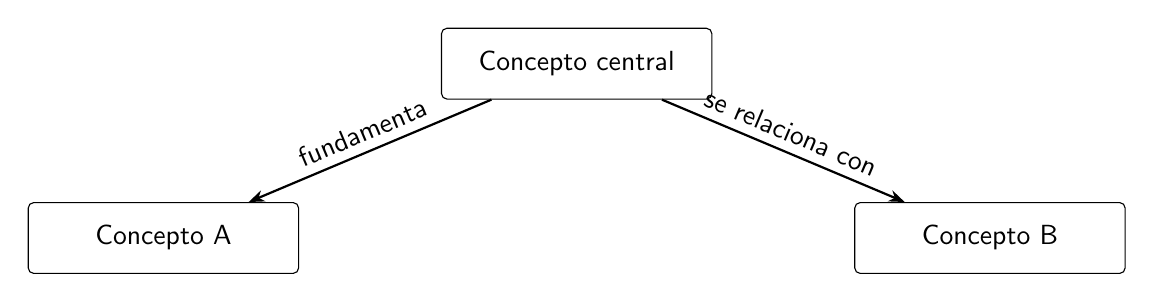
\begin{tikzpicture}[
  concepto/.style={rectangle, draw, rounded corners=2pt,
    align=center, text width=3.2cm, minimum height=0.9cm},
  flecha/.style={-{Stealth[length=2mm]}, thick}
]
\node[concepto] (a) {Concepto central};
\node[concepto, below left=1.3cm and 1.8cm of a] (b) {Concepto A};
\node[concepto, below right=1.3cm and 1.8cm of a] (c) {Concepto B};
\draw[flecha] (a) -- node[above, sloped]{fundamenta} (b);
\draw[flecha] (a) -- node[above, sloped]{se relaciona con} (c);
\end{tikzpicture}
\caption{Mapa conceptual de [tema]}
\end{figure}
\end{verbatim}

\subsubsection*{Línea de tiempo}

\begin{verbatim}
\begin{figure}[H]
\centering
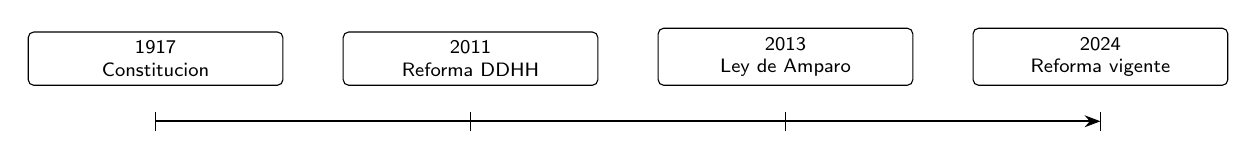
\begin{tikzpicture}[
  evento/.style={rectangle, draw, rounded corners=2pt,
    align=center, text width=3cm, font=\scriptsize},
  eje/.style={-{Stealth[length=2mm]}, thick}
]
\draw[eje] (0,0) -- (12,0);
\foreach \x/\anio/\texto in {
  0/1917/Constitucion,
  4/2011/Reforma DDHH,
  8/2013/Ley de Amparo,
  12/2024/Reforma vigente}
{
  \draw (\x,0.12) -- (\x,-0.12);
  \node[evento, above=0.45cm] at (\x,0) {\anio\\\texto};
}
\end{tikzpicture}
\caption{Linea de tiempo de [tema]}
\end{figure}
\end{verbatim}

\subsubsection*{Diagrama de flujo}

\begin{verbatim}
\begin{figure}[H]
\centering
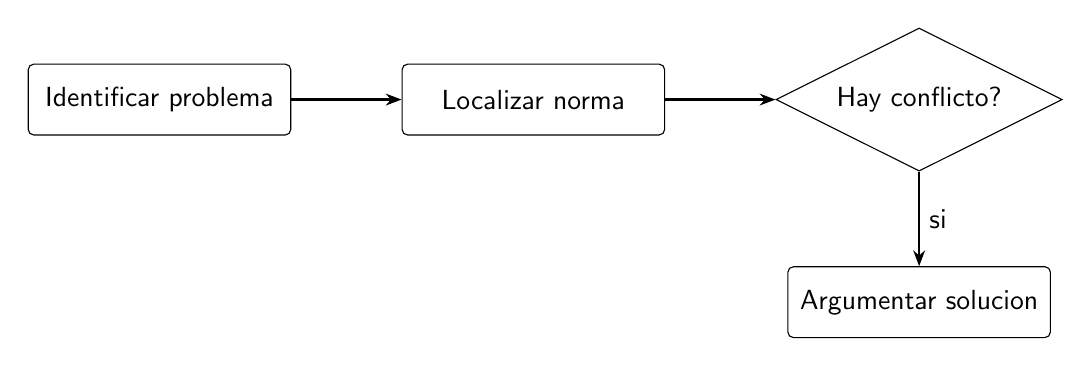
\begin{tikzpicture}[
  paso/.style={rectangle, draw, rounded corners=2pt,
    align=center, text width=3.1cm, minimum height=0.9cm},
  decision/.style={diamond, draw, aspect=2, align=center,
    text width=2.8cm, inner sep=1pt},
  flecha/.style={-{Stealth[length=2mm]}, thick}
]
\node[paso] (inicio) {Identificar problema};
\node[paso, right=1.4cm of inicio] (norma) {Localizar norma};
\node[decision, right=1.4cm of norma] (decision) {Hay conflicto?};
\node[paso, below=1.2cm of decision] (analisis) {Argumentar solucion};
\draw[flecha] (inicio) -- (norma);
\draw[flecha] (norma) -- (decision);
\draw[flecha] (decision) -- node[right]{si} (analisis);
\end{tikzpicture}
\caption{Diagrama de flujo de [proceso]}
\end{figure}
\end{verbatim}

\subsection{Cierre operativo}

La elección de una técnica no debe ser decorativa. Si la actividad pide un producto, la técnica funciona como una herramienta de análisis. El criterio de calidad es que el producto permita ver una decisión intelectual: qué se seleccionó, cómo se organizó, qué relación se construyó y qué postura se puede defender a partir de esa organización.


% ==============================================================================
% REFERENCIAS
% Reglas:
% - Toda fuente citada en el texto debe estar en el .bib.
% - Toda cita debe tener clave correcta.
% - Usar fuentes de la planeacion y, si se complementa, que sean confiables.
% - En el cuerpo: \citep{clave}; no usar solo URLs sueltas.
% ==============================================================================
\bibliography{etica-y-moral-juridica}

% FIN DEL DOCUMENTO
\end{document}


